\PassOptionsToPackage{unicode=true}{hyperref} % options for packages loaded elsewhere
\PassOptionsToPackage{hyphens}{url}
%
\documentclass[openany]{book}
\usepackage{lmodern}
\usepackage{amssymb,amsmath}
\usepackage{ifxetex,ifluatex}
\usepackage{fixltx2e} % provides \textsubscript
\ifnum 0\ifxetex 1\fi\ifluatex 1\fi=0 % if pdftex
  \usepackage[T1]{fontenc}
  \usepackage[utf8]{inputenc}
  \usepackage{textcomp} % provides euro and other symbols
\else % if luatex or xelatex
  \usepackage{unicode-math}
  \defaultfontfeatures{Ligatures=TeX,Scale=MatchLowercase}
\fi
% use upquote if available, for straight quotes in verbatim environments
\IfFileExists{upquote.sty}{\usepackage{upquote}}{}
% use microtype if available
\IfFileExists{microtype.sty}{%
\usepackage[]{microtype}
\UseMicrotypeSet[protrusion]{basicmath} % disable protrusion for tt fonts
}{}
\IfFileExists{parskip.sty}{%
\usepackage{parskip}
}{% else
\setlength{\parindent}{0pt}
\setlength{\parskip}{6pt plus 2pt minus 1pt}
}
\usepackage{hyperref}
\hypersetup{
            pdftitle={CLU MS Clinical Psychology Thesis Handbook},
            pdfauthor={Jamie Bedics, PhD, ABPP, Program Director},
            pdfborder={0 0 0},
            breaklinks=true}
\urlstyle{same}  % don't use monospace font for urls
\usepackage{longtable,booktabs}
% Fix footnotes in tables (requires footnote package)
\IfFileExists{footnote.sty}{\usepackage{footnote}\makesavenoteenv{longtable}}{}
\usepackage{graphicx,grffile}
\makeatletter
\def\maxwidth{\ifdim\Gin@nat@width>\linewidth\linewidth\else\Gin@nat@width\fi}
\def\maxheight{\ifdim\Gin@nat@height>\textheight\textheight\else\Gin@nat@height\fi}
\makeatother
% Scale images if necessary, so that they will not overflow the page
% margins by default, and it is still possible to overwrite the defaults
% using explicit options in \includegraphics[width, height, ...]{}
\setkeys{Gin}{width=\maxwidth,height=\maxheight,keepaspectratio}
\setlength{\emergencystretch}{3em}  % prevent overfull lines
\providecommand{\tightlist}{%
  \setlength{\itemsep}{0pt}\setlength{\parskip}{0pt}}
\setcounter{secnumdepth}{5}
% Redefines (sub)paragraphs to behave more like sections
\ifx\paragraph\undefined\else
\let\oldparagraph\paragraph
\renewcommand{\paragraph}[1]{\oldparagraph{#1}\mbox{}}
\fi
\ifx\subparagraph\undefined\else
\let\oldsubparagraph\subparagraph
\renewcommand{\subparagraph}[1]{\oldsubparagraph{#1}\mbox{}}
\fi

% set default figure placement to htbp
\makeatletter
\def\fps@figure{htbp}
\makeatother

\usepackage{booktabs}
\usepackage{amsthm}
\makeatletter
\def\thm@space@setup{%
  \thm@preskip=8pt plus 2pt minus 4pt
  \thm@postskip=\thm@preskip
}
\makeatother
\usepackage[]{natbib}
\bibliographystyle{apalike}

\title{CLU MS Clinical Psychology Thesis Handbook}
\author{Jamie Bedics, PhD, ABPP, Program Director}
\date{2020-05-22}

\begin{document}
\maketitle

{
\setcounter{tocdepth}{1}
\tableofcontents
}
\hypertarget{goal-of-the-handbook}{%
\chapter{Goal of the Handbook}\label{goal-of-the-handbook}}

\begin{center}\rule{0.5\linewidth}{0.5pt}\end{center}

The goal of this handbook is to provide students with the information needed to successfully complete the master's thesis in the MS in Clinical Psychology Program (MSCP) at California Lutheran University (CLU). The manual should be understood as a supplement to the broader policies and procedures defined by the program and university.

Updates can be found at: \url{https://jdbedics.github.io/thesishandbook/}

\begin{center}\rule{0.5\linewidth}{0.5pt}\end{center}

\hypertarget{scholarly-research}{%
\section{Scholarly Research}\label{scholarly-research}}

\begin{center}\rule{0.5\linewidth}{0.5pt}\end{center}

\textbf{Overview:} Scholarly research requires the skills of scientific inquiry as a method of addressing a problem. As a participant in research activities in the MSCP program, students are expected to develop the following abilities:

\begin{enumerate}
\def\labelenumi{\arabic{enumi}.}
\tightlist
\item
  Create or contribute empirical knowledge to the existing body of information in a discipline.
\item
  Carryout systematic inquiry of a body of literature.
\item
  Use tools of research including analyzing existing research, implementing research designs, using and/or developing instrumentation, employing appropriate methods of data analysis, and handling the logistics of conducting a research study.
\item
  Work with faculty or other professionals on a research project.
\item
  Use scholarly writing techniques including the mastery of the new \href{https://apastyle.apa.org/products/publication-manual-7th-edition/}{APA Publication Manual 7th Edition}.
\item
  Create and share reproducible and transparent research materials including open data and code consistent with the principles of open science.
\end{enumerate}

Research conducted in the MSCP program may be a thesis or a research project. While both are important contributions to the body of knowledge in a discipline, they have different purposes as described in the following sections. The most critical being that the thesis is taken for credit and partial fulfillment of the degree and in replacement of the comprehensive exam.

\begin{center}\rule{0.5\linewidth}{0.5pt}\end{center}

\hypertarget{comprehensive-exam}{%
\section{Comprehensive Exam}\label{comprehensive-exam}}

By default, students entering the MSCP program are required to complete the comprehensive exam. Students can, however, choose to \emph{opt out} of the comprehensive exam and instead complete a thesis.

\textbf{What is the comprehensive exam?}

\begin{itemize}
\tightlist
\item
  A closed book essay test that covers all the material studied during the program.\\
\item
  The test is offered at the end of the spring semester during the second year.
\item
  The exam consists of a morning session (9AM-Noon) and an afternoon session (1PM-4PM).
\item
  During each session, students choose to respond to 3 of 5 questions.
\item
  Students are given a thorough review sheet to facilitate studying for the exam.
\end{itemize}

\textbf{How the comprehensive exam \emph{replaces} the thesis}

\begin{itemize}
\tightlist
\item
  Students register for the exam by paying a \emph{comprehensive exam fee} during the semester they take the exam (typically spring of their 2nd year).
\item
  Students \textbf{do not} take \emph{PSYC 566 Thesis (3 units)} in the spring of their 2nd year.\\
\item
  As a result, students who take the comprehensive exams graduate with a total of \textbf{37-units}
  instead of 40-units with the thesis option.
\item
  Students who take the comprehensive exam are also \textbf{not} required to take \emph{PSYC 565 Research Practicum} in the fall of their 2nd year. Instead, students can choose an elective course in consultation with the Program Director.\footnote{As noted below, students can intend to complete the thesis and take PSYC 565 and PSYC 566 but switch to the comprehensive exam for a variety of reasons. In these cases, students are still required to pay the comprehensive exam fee although they have already paid for thesis units.}
\end{itemize}

\hypertarget{thesis}{%
\section{Thesis}\label{thesis}}

The thesis is the result of an original empirical investigation that creates new knowledge within a discipline. It attempts to address a problem related to lack of knowledge and is generally composed of the following elements:

\begin{enumerate}
\def\labelenumi{\arabic{enumi}.}
\tightlist
\item
  Identification of a problem caused by lack of knowledge;
\item
  Background and literature review of existing information about the problem;
\item
  Methods to be used for obtaining the needed knowledge;
\item
  Resulting new knowledge;
\item
  Interpretation of the new knowledge;
\item
  Transparent and open sharing of materials and results through the use of the open science framework.
\end{enumerate}

\textbf{Tasks:}

\begin{itemize}
\tightlist
\item
  Students complete all the requirements outlined in this manual.
\item
  Students enroll in \textbf{\emph{PSYC 565 Research Practicum (3 units)}} during the fall of their 2nd year.
\item
  Students enroll in \textbf{\emph{PSYC 566 Thesis (3 units)}} during the spring of their 2nd year.
\item
  Students who fail to complete the thesis by the end of the 2nd year can:

  \begin{enumerate}
  \def\labelenumi{\arabic{enumi}.}
  \tightlist
  \item
    Take \textbf{\emph{PSYC 599-01 Thesis Continuation}} and pay all associated fees every semester until the thesis is completed or,
  \item
    Take the comprehensive exam and pay the comprehensive exam fee in the semester immediately following the last semster thesis units were taken.
  \end{enumerate}
\end{itemize}

\hypertarget{research-project-option}{%
\section{Research Project Option}\label{research-project-option}}

\textbf{Research Project + Comprehensive Exam}

Students can complete their own independent research project, identical to the thesis, but without the coursework (PSYC 565 or PSYC 566) and obligation to follow the requirements in this manual. There are two scenarios where a student might choose to take the comprehensive exam and work on a research project :

\begin{enumerate}
\def\labelenumi{\arabic{enumi}.}
\item
  A student can decide, from the beginning of the program, that they want to avoid the pressure and extra work of the thesis requirements but use the program to work on an research project at their own pace and with faulty support. They could take PSYC 565 in the fall of their second year to support their research project but will not take PSYC 566 during the spring. In this case, PSYC 565 will act as their elective.
\item
  Students might attempt the thesis but, for a variety of reasons, fall behind and not be able to complete all the necessary requirements of the thesis in order to graduate. If this occurs, then the student can always move to the comprehensive exam (in order to graduate) while continuing to work on their thesis as an independent research project (for no credit).
\end{enumerate}

In both of these scenarios, students are required to take the comprehensive exam and pay the comprehensive exam fee in order to graduate.

\begin{center}\rule{0.5\linewidth}{0.5pt}\end{center}

\hypertarget{pros-and-cons-thesis-vs.-comps}{%
\section{Pros and Cons: Thesis Vs. Comps}\label{pros-and-cons-thesis-vs.-comps}}

\textbf{\emph{Thesis ``Pros''}}

\begin{itemize}
\tightlist
\item
  Students gain a high degree of expertise and mastery in the area under study.
\item
  The thesis timeline creates accountability and structure in completing the thesis.
\item
  Doctoral programs often look favorably towards a completed thesis that demonstrates students' ability to successfully complete a research project.
\item
  Doctoral programs that require a thesis might \emph{waive} the thesis requirement based upon the completed thesis at CLU.
\item
  Students can have the thesis bound into a book (see \protect\hyperlink{binding}{Section 6 Thesis Binding}).
\item
  Students can earn quality letters for recommendation from their thesis committee members. These letters are often more meaningful than letters from employers or course instructors.
\end{itemize}

\textbf{\emph{Thesis ``Cons''}}

\begin{itemize}
\tightlist
\item
  Despite the structure offered through coursework, the thesis requires a considerable amount of extra work and self-discipline. The amount of autonomy and work can be quite stressful.
\item
  Students take an extra 3-units (PSYC 566) in the spring of their 2nd year for a total of 40-units versus 37-units for the comprehensive exam option.
\end{itemize}

\begin{center}\rule{0.5\linewidth}{0.5pt}\end{center}

\textbf{\emph{Comps ``Pros''}}

\begin{itemize}
\tightlist
\item
  Students are given a review sheet to help them study.
\item
  The exam is completed in a single day compared to the thesis that takes 2-years.
\item
  Questions that are not adequately answered can be successfully remitted before ``failing.''
\item
  Students can still complete an \textbf{research project} (see next section) which would allow the first three \emph{thesis pros} to be achieved. A good research project is just as valued as a good thesis.
\item
  Students can choose any 3-credit elective during their second year (spring is recommended).
\item
  The entire program is \textbf{37-units} versus 40-units with the thesis option.
\end{itemize}

\textbf{\emph{Comps ``Cons''}}

\begin{itemize}
\tightlist
\item
  A 6-hour, closed book, essay test can be stressful and exhausting.
\item
  Research experience is valued by PHD programs and many, but not all, PSYD programs.
\item
  The research project, if chosen, could not be as structured as the thesis option.
\end{itemize}

\begin{center}\rule{0.5\linewidth}{0.5pt}\end{center}

\hypertarget{thesis-checklist---overview}{%
\chapter{Thesis Checklist - Overview}\label{thesis-checklist---overview}}

Students who wish to pursue the thesis option are required to meet with Dr.~Bedics at the end of every semester in order to review their progress according to the following timeline. Students who miss any of the following steps are removed from the thesis option and will be required to complete the comprehensive exam in order to graduate.

\begin{longtable}[]{@{}lllll@{}}
\toprule
& Task & Date Due & Year & Finished\tabularnewline
\midrule
\endhead
1. & Thesis Topic Approved & October 1st & First Year & {[}\_\_\_\_\_{]}\tabularnewline
2. & Setup OSF & October 1st & First Year & {[}\_\_\_\_\_{]}\tabularnewline
3. & Literature Review Draft Psych 564 & December 15th & First Year & {[}\_\_\_\_\_{]}\tabularnewline
4. & Academic Good Standing & December 15th & First Year & {[}\_\_\_\_\_{]}\tabularnewline
5. & Method Section Draft & May 1st & First Year & {[}\_\_\_\_\_{]}\tabularnewline
6. & Literature Review Revision & May 1st & First Year & {[}\_\_\_\_\_{]}\tabularnewline
7. & Academic Good Standing & May 15th & First Year & {[}\_\_\_\_\_{]}\tabularnewline
8. & Committee Assignment & June 30th & Summer & {[}\_\_{]} Chair{[}\_\_{]} Reader\tabularnewline
9. & Academic Good Standing & July 3rd & Summer & {[}\_\_\_\_\_{]}\tabularnewline
10. & Enroll in PSYC 565 & August 1st & Second Year & {[}\_\_\_\_\_{]}\tabularnewline
11. & Committee Approval of Proposal & September 1st & Second Year & {[}\_\_\_\_\_{]}\tabularnewline
12. & IRB Submitted & November 1st & Second Year & {[}\_\_\_\_\_{]}\tabularnewline
13. & Academic Good Standing & December 15th & Second Year & {[}\_\_\_\_\_{]}\tabularnewline
14. & Enroll in PSYC 566 & December 15th & Second Year & {[}\_\_\_\_\_{]}\tabularnewline
15. & Complete Draft to Dr.~Bedics & May 1st & Second Year & {[}\_\_\_\_\_{]}\tabularnewline
16. & Committee Approval of Final & May 10th & Second Year & {[}\_\_{]} Chair{[}\_\_{]} Reader\tabularnewline
17. & OSF Approval & May 1st & Second Year & {[}\_\_\_\_\_{]}\tabularnewline
18. & Thesis Commons & May 15th & Second Year & {[}\_\_\_\_\_{]}\tabularnewline
19. & Thesis Binding & Optional & Second Year & {[}\_\_\_\_\_{]}\tabularnewline
20. & GitHub Blog & Optional & Second Year & {[}\_\_\_\_\_{]}\tabularnewline
21. & Shiny App & Optional & Second Year & {[}\_\_\_\_\_{]}\tabularnewline
\bottomrule
\end{longtable}

\hypertarget{thesis-topic-selection}{%
\section{Thesis Topic Selection}\label{thesis-topic-selection}}

\begin{center}\rule{0.5\linewidth}{0.5pt}\end{center}

\textbf{Defining the Problem Area}

The general thesis topic is required to be selected during the beginning of the first semester of the first year. The thesis topic, does not, however, determine the hypotheses, methodology or general approach taken by the student to understand the problem (e.g.~experimental, quasi-experimental, meta-analytic methods). It would be premature for any student to attempt to define a hypothesis in the first year when their understanding of the topic area is limited and not justified by a thorough literature review. Hypotheses are typically developed after the first year of study when the student has a better grasp of the problem to be solved (see the Wampold article in \protect\hyperlink{resources}{Section 10 References} for a guide on hypothesis development).

\begin{center}\rule{0.5\linewidth}{0.5pt}\end{center}

\textbf{\emph{Tips for finding a Topic}}

Students are often unnecessarily delayed in choosing a broad area to study which can impact the success of the thesis. In choosing a topic students should keep a few points in mind:

\begin{enumerate}
\def\labelenumi{\arabic{enumi}.}
\item
  It certainly is helpful if you are \textbf{passionate} about the topic. When a person is passionate about a topic they naturally want to read about and understand the area under study. They often go to bed thinking about the topic and will wake up excited and thinking about what they will do that day related to their project. It can be a very exciting time because you're working on something you love and have fun doing.
\item
  \textbf{Reflect on your interests.} It's okay if you are not particularly passionate about any specific area of study. Passion often starts by first examining an area of \textbf{interest} with some degree of focus, commitment, and consistency. If you have an area of interest then the next step is to simply select one area, commit to it, and start reading and writing. Passion often comes \emph{after} we put the work in.
\item
  \textbf{Select \emph{one} interest. Don't flip-flop.} The problem is that we all have multiple interests. For example, you might really like schizophrenia but at the same time you're really interested in forensic psychology and the prison system. One semester you might want to study psychosis and the next semester you might become more interested in the prison system. Students can ``flip flop'' for a variety of reasons which can have two unfortunate consequences. First, you never get anything done. When you don't get anything done then it's hard to feel good about yourself and you make no progress. Second, continued indecisiveness could implicitly instill in the student a sense that they should always feel comfortable with their topic, that work on the thesis should always be easy and interesting, or that they might be ``missing out'' by not researching some other area of interest. In reality, none of these are true. One of the greatest challenges of doing research is developing the ability to consistently make small steps on a project even when the feeling is not there or other demands are present and taking up our time. It is likely that you're lifestyle and habits will change when dedicated to research. You just work more (much, much, more).
\item
  \textbf{The thesis will not define you.} Students should understand that the topic they select to study will not define their career. In this sense, the thesis topic itself is not really that important. What is more important is that students pick a topic so they can learn \emph{how} to do competent research. You can't do that if you don't have a focused topic. In sum, it would be nice if you are passionate or, at minimum, interested in the topic but it simply is not \textbf{\emph{necessary}}.
\item
  \textbf{Find an article that excites you.} One way to find a topic is to choose an area of interest and read as many research articles in the subject that you can. In doing so, it will be easiest to read the introduction and discussion sections only. Diving into the method and results can sometimes be overwhelming and demoralizing. Once a student finds an article that excites them, they can consider the method and results section. A second important point here is that good science should include \textbf{replication}. An excellent thesis would be a replication study to see if the effects reported in prior work can be found again. We do not often do this in psychological science and our field suffers because of it.
\end{enumerate}

\textbf{Due}: October 1st, first year.

\begin{center}\rule{0.5\linewidth}{0.5pt}\end{center}

\hypertarget{open-science-framework}{%
\section{Open Science Framework}\label{open-science-framework}}

\textbf{Creating a transparent and reproducible workflow}


\includegraphics{images/osf.png}

\href{https://osf.io/}{OSF} is a repository that allows researchers to transparently share their work with the larger scientific community. During the course of the program, students use OSF to organize their thesis and other independent research projects. Instructions for setting up an OSF project can be found \href{https://speakerdeck.com/jdbedics/osf-setup-and-class-project-introduction}{here} and will be reviewed with Dr.~Bedics at students first advising meeting.

In addition to organizing students' workflow, OSF allows students to showcase their work to their peers and potential employers and doctoral advisors. Students in the thesis option are required to use OSF and it is strongly recommended for students completing the research project.

\textbf{Due}: October 1st, first year.

\begin{center}\rule{0.5\linewidth}{0.5pt}\end{center}

\hypertarget{literature-review-timeline}{%
\section{Literature Review Timeline}\label{literature-review-timeline}}

\begin{center}\rule{0.5\linewidth}{0.5pt}\end{center}

\textbf{Understanding the Problem}

The development of the literature review begins during the fall of the first year during PSYC 564 Advanced Research Methods. The literature review will become the ``introduction'' section of the final thesis paper. The literature review demonstrates the student's mastery of the literature surrounding the \emph{problem} to be addressed by the thesis. Initial drafts, such as that from PSYC 564, are 10-12 pages in length.

The development of the literature review is, however, ongoing throughout the two years of the program until the final draft is submitted on May 1st of the second year. The typical length of a \emph{completed} introduction section is between \textbf{20-40 pages} long but there is no maximum length.

In terms of content, students are encouraged to consider multiple perspectives in their work and also to integrate their thoughts related to culture and diversity regarding the topic area. The idea here is that a good understanding of a problem area involves a thorough understanding of the context. Context includes a consideration of the place, time, and people under study as well as the same characteristics of those who are doing the investigating.

\textbf{Due}:

\begin{enumerate}
\def\labelenumi{\arabic{enumi}.}
\tightlist
\item
  December 15th, first year (First Major Draft);
\item
  May 15th, end of first year (Second Major Draft with Hypotheses);
\item
  May 1st, end of second year (Final Draft).
\end{enumerate}

\begin{center}\rule{0.5\linewidth}{0.5pt}\end{center}

\hypertarget{method-section-timeline}{%
\section{Method Section Timeline}\label{method-section-timeline}}

\begin{center}\rule{0.5\linewidth}{0.5pt}\end{center}

\textbf{Solving the Problem}

The method sections defines the procedures of the thesis. The method section consists of the participant selection, selection of methods of measurements or materials, the procedure and the data analytic method. The method section can be worked on in \emph{PSYC 552 Psychometrics} during spring of the first year and also \emph{PSYC 562 Statistics II: Regression.} The method section is finalized during \emph{PSYC 565 Research Practicum} in the fall of the second year.

Lastly, the method section should include a \textbf{power analysis.} The primary purpose of the power analysis is to provide students with the best understanding of the size of the sample needed to successfully test their hypothesis. In other words, students should never have to say in their discussion ``The study was limited due to a small sample. Future research should include a larger sample size.'' When authors make this statement they are basically stating that they ran a study where they can't lose. If they find significance then great. If they don't then they say ``Oh well, we're probably right but just need more people.'' You should ask yourself, why would you run a test when you couldn't reach a conclusion and when you basically say you ``win'' regardless. It makes no sense to run the study.

The power analysis should be calculated during the summer or during PSYC 565 in the fall of the second year and prior to IRB submission.

\textbf{Video Resources:}

\begin{enumerate}
\def\labelenumi{\arabic{enumi}.}
\item
  A conceptual overview of power analysis can be found \href{https://www.youtube.com/watch?v=Lr-i4Ugoc5M}{here}. If you like that professor, here is another video by him that I like on his personal \href{https://www.youtube.com/watch?v=XhfkodpyIsw}{website}
\item
  An overview from the Center for Open Science.
\end{enumerate}

\href{https://www.youtube.com/watch?v=-ZU7fbvSJ60}{Part 1, What is Statisical Power}
\href{https://www.youtube.com/watch?v=7daQRvRO-NE}{Part 2, Consequences of low power}

Any article on the topic can found in the \protect\hyperlink{resources}{10 Resources}

\textbf{Due}:

\begin{enumerate}
\def\labelenumi{\arabic{enumi}.}
\tightlist
\item
  May 1st, first year (First Draft);
\item
  December 15th, second year (Second Draft including power analysis)
\end{enumerate}

\begin{center}\rule{0.5\linewidth}{0.5pt}\end{center}

\hypertarget{committee-assignment}{%
\section{Committee Assignment}\label{committee-assignment}}

\begin{center}\rule{0.5\linewidth}{0.5pt}\end{center}

Committee members are faculty or experts in the field that support the students work on the thesis. Students work with the program director to find the most appropriate committee members to support their research project. The committee is composed of a Chair and a Reader. Their roles are described below as is the process for finding and selecting committee members.

\begin{center}\rule{0.5\linewidth}{0.5pt}\end{center}

\textbf{Committee Chair}

The chair must have \emph{content knowledge} of the area under investigation for the thesis. For example, if the thesis is on schizophrenia then the chair must have extensive knowledge of schizophrenia. The chair is either a part-time or full-time faculty member at CLU and is chosen with the approval of the Program Director, Dr.~Bedics. There can be exceptions to the above criteria with the approval of Dr.~Bedics.

\textbf{Committee Reader}

The reader must have either content knowledge or expert \emph{methodological knowledge} of the area under investigation for the thesis. For example, if the thesis is on schizophrenia and utilizes an experimental design then the reader can either have knowledge of schizophrenia \textbf{or} knowledge of the experimental methods proposed. The reader can be a part-time or full-time faculty member at CLU or a professional in the community with at least a Master's degree that has the aforementioned expertise. The reader must be chosen with approval of Program Director and thesis Committee Chair. There can be exceptions to the above criteria with the approval of Dr.~Bedics.

\begin{center}\rule{0.5\linewidth}{0.5pt}\end{center}

Please see \protect\hyperlink{people}{Section 4 Thesis Committee} of this handbook for information on how to acquire a committee.

\textbf{Due}: June 30th, Summer after First Year

\begin{center}\rule{0.5\linewidth}{0.5pt}\end{center}

\hypertarget{committee-approval-of-proposal}{%
\section{Committee Approval of Proposal}\label{committee-approval-of-proposal}}

\begin{center}\rule{0.5\linewidth}{0.5pt}\end{center}

During the summer following the first year, committee members read the literature review and method section and provide a general statement of approval to Dr.~Bedics. Based upon this approval, students are allowed to progress to the \textbf{thesis track} and enroll in PSYC 565 Research Practicum in the fall of the second year and PSYC 566 Thesis in the spring of the second year.

\textbf{Due}: September 1st, Second Year

\begin{center}\rule{0.5\linewidth}{0.5pt}\end{center}

\hypertarget{academic-good-standing}{%
\section{Academic Good Standing}\label{academic-good-standing}}

\begin{center}\rule{0.5\linewidth}{0.5pt}\end{center}

Academic good standing refers to maintaining a GPA above a 3.0 throughout the entire program and acting consistently with all policies and procedures defined by the program (see Program Handbook) and university (see university policy and procedures). Any student who receives below a B- in any course, at anytime in the program, is not allowed to complete the thesis for course credit and partial fulfillment of the degree. They can, however, complete a research project with the support of full-time faculty.

\textbf{Due}: Every semester

\begin{center}\rule{0.5\linewidth}{0.5pt}\end{center}

\hypertarget{format-of-paper---overview}{%
\chapter{Format of Paper - Overview}\label{format-of-paper---overview}}

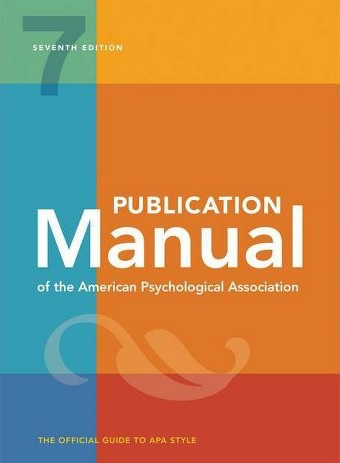
\includegraphics{images/apamanual.png}

The thesis paper is completed in a manner consistent with the \href{https://www.amazon.com/s?k=apa+publication+manual+7th+edition\&crid=7T10VJ2PYQZH\&sprefix=apa+pu\%2Caps\%2C261\&ref=nb_sb_ss_i_1_6}{Publication Manual of the APA (7th Edition)}.\footnote{* Sections with asterisks \textbf{do not} follow APA style}

\begin{itemize}
\tightlist
\item
  Title Page*
\item
  Signature Page*
\item
  Dedication*
\item
  Acknowledgements*
\item
  Table of Contents*
\item
  Abstract
\item
  Introduction
\item
  Method
\item
  Results
\item
  Discussion
\item
  References
\item
  Tables
\item
  Figures
\item
  Appendices
\end{itemize}

\hypertarget{title-page}{%
\section{Title Page}\label{title-page}}

This page provides the name of the thesis project, names of the university and school or department, and date of completion. The title page should be prepared in accordance with the sample page found in this section. The date at the bottom of the page is the month and year the degree is awarded. The title page is unnumbered but is counted as page ``i.''

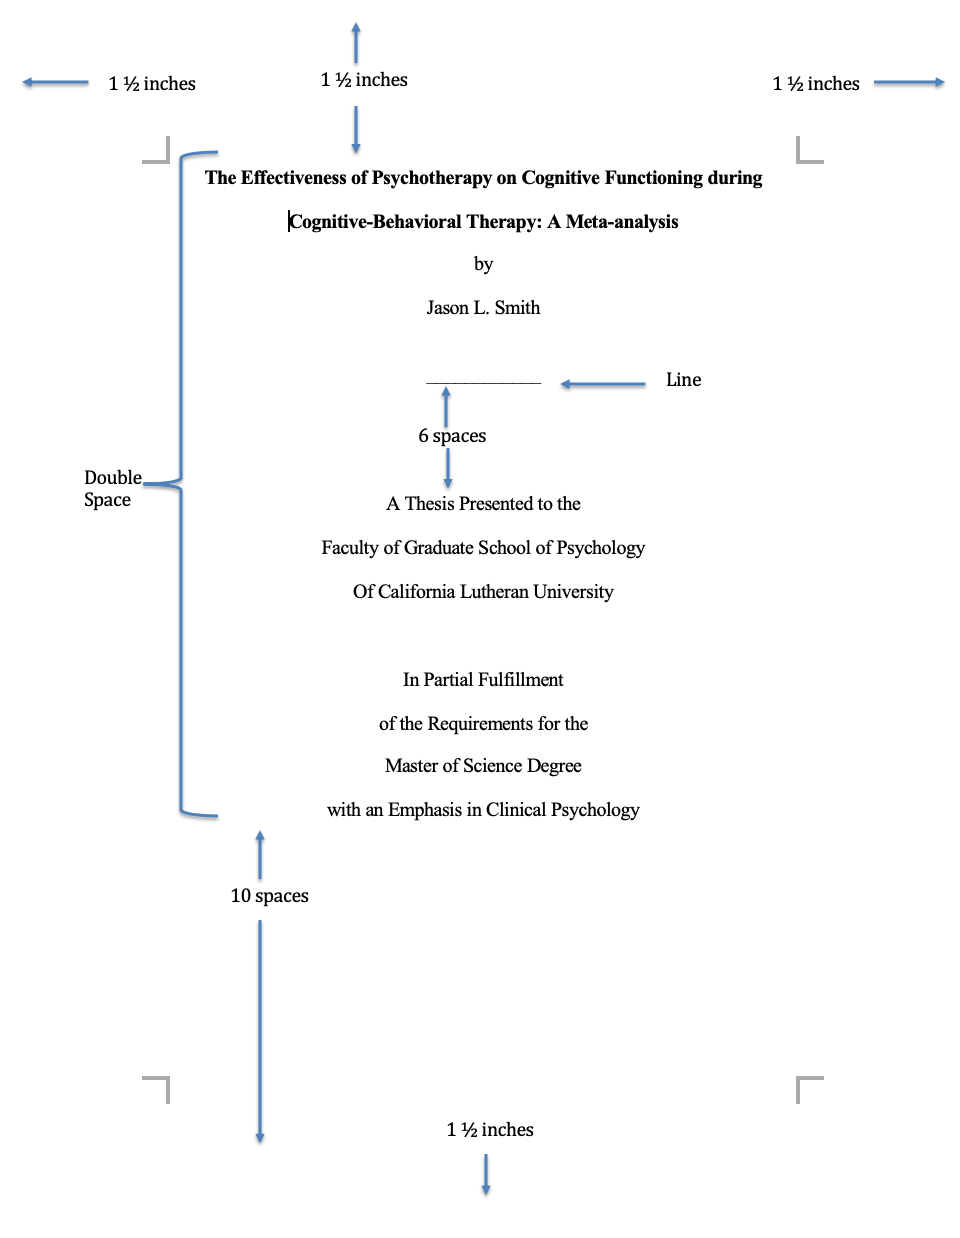
\includegraphics{images/titlepage.png}

\begin{center}\rule{0.5\linewidth}{0.5pt}\end{center}

\hypertarget{signature-page}{%
\section{Signature Page}\label{signature-page}}

This page provides the name of the author and blank lines for the signatures of the committee members and the Graduate Dean of the appropriate School. The pages are signed when the members and Dean determine that the thesis or project is complete. The approval page should comply with the page form found in Appendix B. It should bear original signatures for all copies. The date at the bottom of the page is the date the degree is awarded; however, the page is not counted in the numbering system.

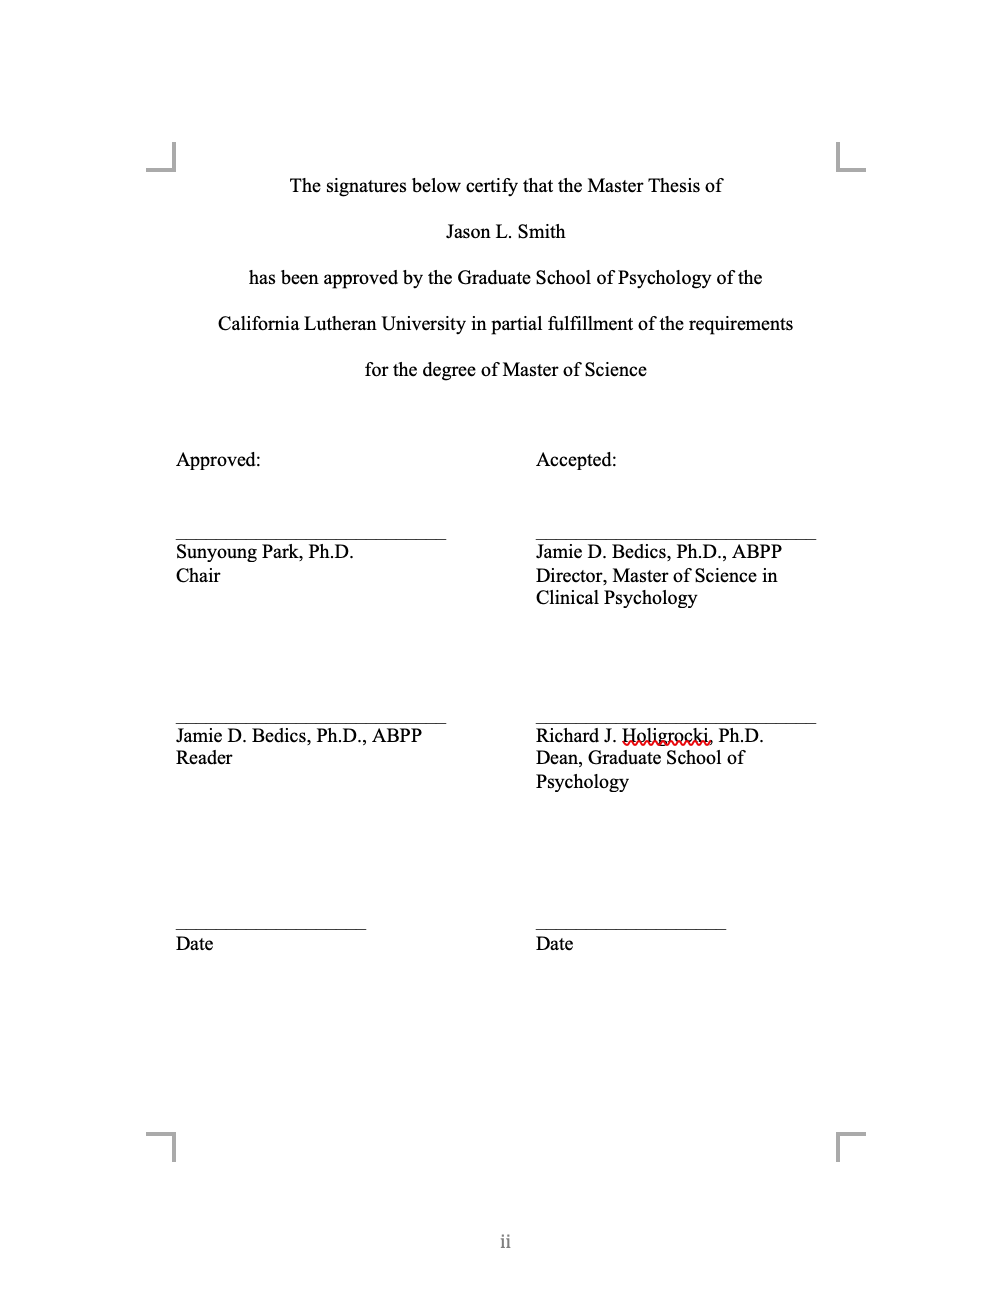
\includegraphics{images/signaturepage.png}

\begin{center}\rule{0.5\linewidth}{0.5pt}\end{center}

\hypertarget{dedication-optional}{%
\section{Dedication (optional)}\label{dedication-optional}}

This optional page contains a brief dedication to the individual(s) whom the author wishes to honor. If included, this page is numbered as page ``ii'' (lower case Roman numeral).

\begin{center}\rule{0.5\linewidth}{0.5pt}\end{center}

\hypertarget{acknowledgements-optional}{%
\section{Acknowledgements (optional)}\label{acknowledgements-optional}}

This optional page lists persons and/ or institutions whom the author wishes to thank for their assistance in completing the thesis or project. Such assistance can be provision of personal, financial, or moral support, or access to data sets or subject populations. A brief statement as to the type of assistance provided may follow each person or institution named. If included, this page continues the lower case Roman numeral sequence begun above.

\begin{center}\rule{0.5\linewidth}{0.5pt}\end{center}

\hypertarget{table-of-contents}{%
\section{Table of Contents}\label{table-of-contents}}

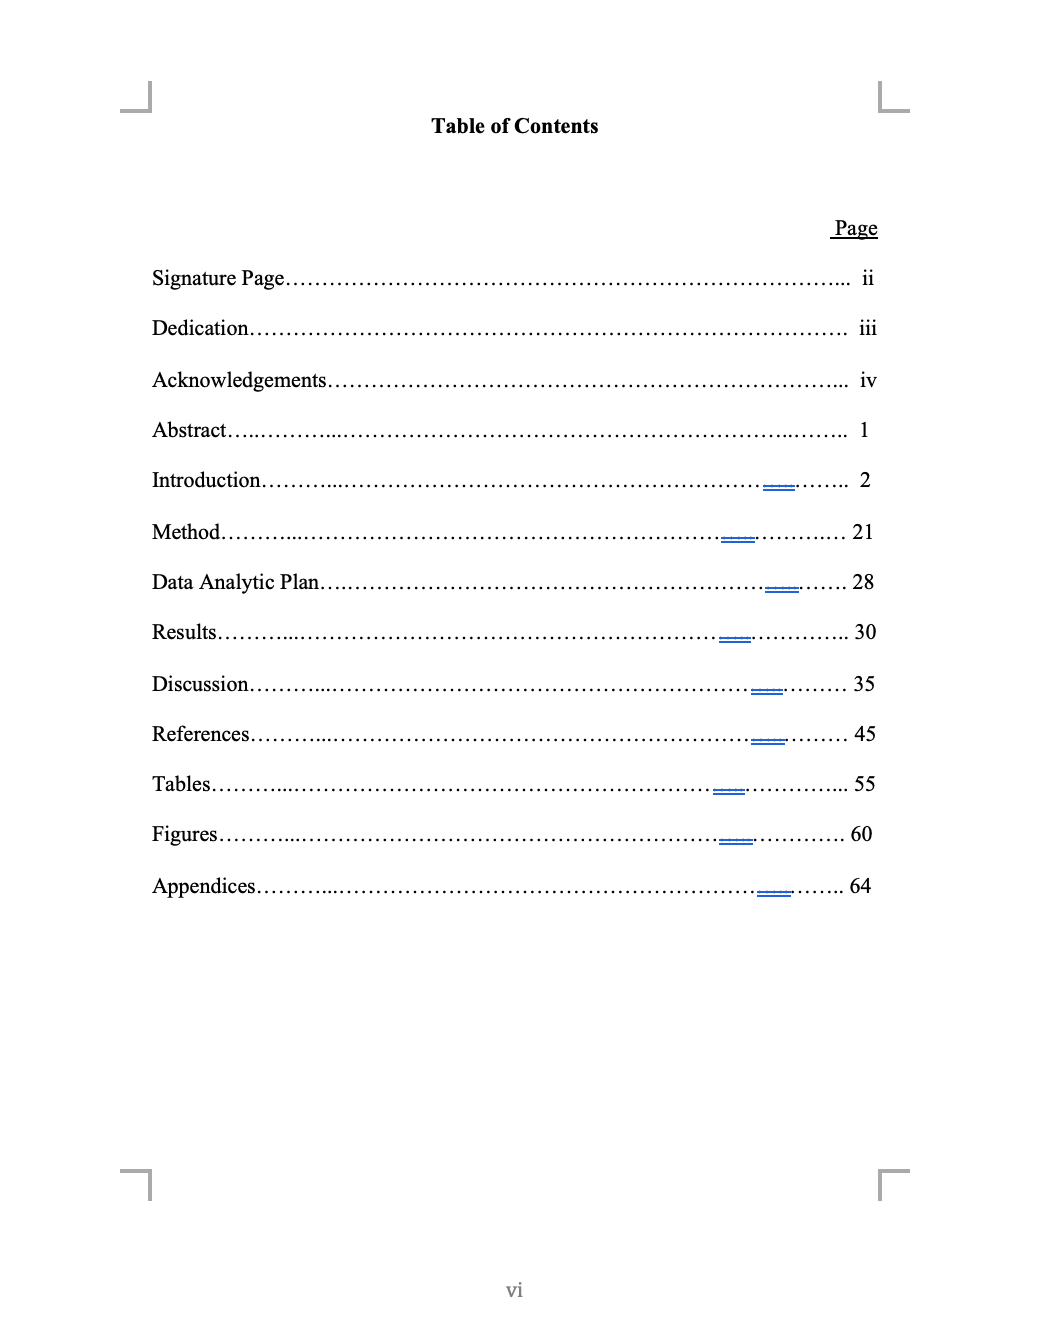
\includegraphics{images/tablecontents.png}

\begin{center}\rule{0.5\linewidth}{0.5pt}\end{center}

\hypertarget{abstract-apa-style}{%
\section{Abstract (APA style)}\label{abstract-apa-style}}

The abstract follows APA style and typically completed in the spring of the second semester. A draft of the abstract, without results and without concluding statements, might be drafted during \emph{PSYC 565 Research Practicum} during the of the second year.

\begin{center}\rule{0.5\linewidth}{0.5pt}\end{center}

\hypertarget{introduction-apa-style}{%
\section{Introduction (APA style)}\label{introduction-apa-style}}

As noted in the section ``Literature Review Timeline,'' the introduction is drafted during the first semester of the first year in \emph{PSYC 564} and revised every semester of the year. The introduction is a comprehensive document that demonstrates the students' expertise in the area under study. A good introduction demonstrated understanding. In many theses, understanding involves an appreciation and discussion of culture and diversity and a literature review would be incomplete without such a review.

\begin{center}\rule{0.5\linewidth}{0.5pt}\end{center}

\hypertarget{method-apa-style}{%
\section{Method (APA style)}\label{method-apa-style}}

As noted in the ``Method Section Timeline,'' portions of the Method section can be drafted during the spring semester and finalized during PSYC 565 in the fall of the second year. The method section defines the procedures of the study and is required for successful IRB approval at CLU. IRB is accomplished during PSYC 565 in the of the second year but students should review CLU IRB requirements as soon as possible. A link to the CLU IRB can be found here: \url{https://www.callutheran.edu/research/irb/}.

\begin{center}\rule{0.5\linewidth}{0.5pt}\end{center}

\hypertarget{data-analytic-method-apa-style}{%
\section{Data Analytic Method (APA style)}\label{data-analytic-method-apa-style}}

The data analytic plan can be developed during PSYC 562 in the spring of the first year and finalized during PSYC 565 in the of the second year. At CLU, we exclusively use the statistical program language called R. The data analytic section will include a power analysis as well a link to the study's pre-registration of the data analysis.

\begin{center}\rule{0.5\linewidth}{0.5pt}\end{center}

\hypertarget{results-apa-style}{%
\section{Results (APA style)}\label{results-apa-style}}

The results are typically drafted during the spring of second year. \emph{PSYC 566 Thesis} is an independent study unit and there are no class meetings. Instead, students meet with their thesis chair to review and write their analyses in the results section.

\begin{center}\rule{0.5\linewidth}{0.5pt}\end{center}

\hypertarget{discussion-apa-style}{%
\section{Discussion (APA style)}\label{discussion-apa-style}}

The discussion is a critical section of the research paper and is typically \textbf{10-pages} minimum. In the discussion the student provide the following:

\begin{itemize}
\tightlist
\item
  A summary of the proposed hypotheses and rationale.
\item
  A review of the results in narrative form without the presentation of any statistics.
\item
  A discussion of the implications of the results for each hypothesis.
\item
  A discussion of future steps for each hypothesis.
\item
  A discussion of the limitations of the study in addressing each hypothesis.
\item
  Similar to the introduction, please consider culture and diversity in your discussion of the findings.
\end{itemize}

The discussion section demonstrates the student's ability to place their study in the context of the larger literature and think more philosophically. It is a space for creativity and ingenuity.

\begin{center}\rule{0.5\linewidth}{0.5pt}\end{center}

\hypertarget{references-apa-style}{%
\section{References (APA style)}\label{references-apa-style}}

References follow APA style. Please make sure all in-text citations are in the reference section and all citations in the reference section are cited in the text.

\begin{center}\rule{0.5\linewidth}{0.5pt}\end{center}

\hypertarget{tables-figures-appendices-apa-style}{%
\section{Tables, Figures, \& Appendices (APA style)}\label{tables-figures-appendices-apa-style}}

Tables and Figures can be essential for helping a reader understand your data analysis and conclusions. Please follow APA formatting for all Table and Figures.

If students choose to bind their thesis then they pay careful attention to formatting in order to maintain the margins of the paper (1.5" all around). This can especially be a problem for Tables.

Appendices often include a student's curriculum vita, IRB approval form, and other materials.

\begin{center}\rule{0.5\linewidth}{0.5pt}\end{center}

\hypertarget{people}{%
\chapter{Thesis Committee}\label{people}}

\textbf{Finding a Committee}

For many faculty, being on a thesis committee is a lot of work and they are often reluctant to agree to help students. Consequently, how students choose to approach faculty is very critical. Please consider these guidelines and talk to Dr.~Bedics prior to reaching out to potential committee members.

\begin{center}\rule{0.5\linewidth}{0.5pt}\end{center}

\textbf{1. Identifying Potential Faculty}

Search the CLU website for potential faculty that could contribute to your idea. Look at faculty interests in graduate psychology, undergraduate psychology, as well as other departments at CLU. Students could also identify faculty at other universities that might serve on the committee. Once identified, students should email Dr.~Bedics to discuss.

\begin{center}\rule{0.5\linewidth}{0.5pt}\end{center}

\textbf{2. Foot-in-the-Door}

Students first introduce themselves to faculty through email. \textbf{Do not ask them to join your committee} in the first email. Instead, ask them if they have time to answer questions about your project. If they don't have time or incentive to do this then they will not be willing to be on your committee. The foot-in-the-door strategy also allows students to gain feedback from the person even if they are not willing to be on students' committee.

Here is a properly formatted and professional email using the foot-in-the-door strategy:

\begin{verbatim}
Dear Dr. ###,

My name is <STUDENT> and I am currently developing my master’s thesis project at California Lutheran University in the MS Clinical Psychology Program.  The topic is <TOPIC>. I think your expertise in <AREA> would help me in thinking through some of the details of the thesis.  I was curious if you could make time to answer a few questions over email or perhaps even chat over the phone or during your office hours?  I have attached a brief summary of my project.

Thank you for your time and consideration.

Sincerely,

First Name Last Name
\end{verbatim}

If they reply, and are positive, then you it is your responsibility to be flexible with \emph{your} time. Also, please never ask for an appointment in the same week.

\begin{center}\rule{0.5\linewidth}{0.5pt}\end{center}

\textbf{3. Requesting Committee Membership} -- If the initial meeting goes well then Dr.~Bedics will email the faculty member to discuss the role of the chair and reader.

\begin{center}\rule{0.5\linewidth}{0.5pt}\end{center}

\textbf{4. Working with your committee}

The committee will be most successful when students establish clear expectations for meeting with their committee members. Clearly established expectations will prevent you from emailing \emph{too little} or \emph{too much}. It is best to suggest \emph{fewer} meetings, perhaps one at the beginning and one at the end of the semester. You will have more meetings with your chair than your reader. Establish the following:

\begin{itemize}
\item
  Make a clear statement that you are respectful of their time and do not want to meet too much or too little. Faculty often appreciate such direct and respectful statements.
\item
  Suggest two meetings a semester and go from there. They might suggest more or a timeline based upon other criteria.
\end{itemize}

\begin{center}\rule{0.5\linewidth}{0.5pt}\end{center}

\hypertarget{coursework-relevant-to-the-thesis}{%
\chapter{Coursework Relevant to the Thesis}\label{coursework-relevant-to-the-thesis}}

\begin{center}\rule{0.5\linewidth}{0.5pt}\end{center}

The knowledge gained from every course taken at CLU can be used to improve the development of the thesis. For example, if you have an interest in examining a specific disorder for your thesis then it makes sense that you study that disorder in \emph{PSYC 510 Psychopathology}. In \emph{PSYC 560 Statistics I: Exploratory Data Analysis}, you might consider finding open data that allows you to better understand your problem area through data visualization.

There are, however, specific courses where the thesis is explicitly incorporated into course assignments. The following are the MSCP courses that explicitly incorporate elements of the thesis into the syllabi:

\begin{longtable}[]{@{}lllll@{}}
\toprule
\begin{minipage}[b]{0.03\columnwidth}\raggedright
PSYC\#\strut
\end{minipage} & \begin{minipage}[b]{0.27\columnwidth}\raggedright
Course\strut
\end{minipage} & \begin{minipage}[b]{0.26\columnwidth}\raggedright
Semester\strut
\end{minipage} & \begin{minipage}[b]{0.10\columnwidth}\raggedright
Year\strut
\end{minipage} & \begin{minipage}[b]{0.19\columnwidth}\raggedright
Task\strut
\end{minipage}\tabularnewline
\midrule
\endhead
\begin{minipage}[t]{0.03\columnwidth}\raggedright
564\strut
\end{minipage} & \begin{minipage}[t]{0.27\columnwidth}\raggedright
Adv. Research Methods\strut
\end{minipage} & \begin{minipage}[t]{0.26\columnwidth}\raggedright
Fall\strut
\end{minipage} & \begin{minipage}[t]{0.10\columnwidth}\raggedright
One\strut
\end{minipage} & \begin{minipage}[t]{0.19\columnwidth}\raggedright
Start Lit Review; Start References\strut
\end{minipage}\tabularnewline
\begin{minipage}[t]{0.03\columnwidth}\raggedright
562\strut
\end{minipage} & \begin{minipage}[t]{0.27\columnwidth}\raggedright
Statistics II: Regression\strut
\end{minipage} & \begin{minipage}[t]{0.26\columnwidth}\raggedright
Spring\strut
\end{minipage} & \begin{minipage}[t]{0.10\columnwidth}\raggedright
One\strut
\end{minipage} & \begin{minipage}[t]{0.19\columnwidth}\raggedright
Data Analytic Plan\strut
\end{minipage}\tabularnewline
\begin{minipage}[t]{0.03\columnwidth}\raggedright
552\strut
\end{minipage} & \begin{minipage}[t]{0.27\columnwidth}\raggedright
Psychometrics\strut
\end{minipage} & \begin{minipage}[t]{0.26\columnwidth}\raggedright
Spring\strut
\end{minipage} & \begin{minipage}[t]{0.10\columnwidth}\raggedright
One\strut
\end{minipage} & \begin{minipage}[t]{0.19\columnwidth}\raggedright
Method\strut
\end{minipage}\tabularnewline
\begin{minipage}[t]{0.03\columnwidth}\raggedright
521\strut
\end{minipage} & \begin{minipage}[t]{0.27\columnwidth}\raggedright
Ethics\strut
\end{minipage} & \begin{minipage}[t]{0.26\columnwidth}\raggedright
Summer\strut
\end{minipage} & \begin{minipage}[t]{0.10\columnwidth}\raggedright
One\strut
\end{minipage} & \begin{minipage}[t]{0.19\columnwidth}\raggedright
Pre-Registration\strut
\end{minipage}\tabularnewline
\begin{minipage}[t]{0.03\columnwidth}\raggedright
565\strut
\end{minipage} & \begin{minipage}[t]{0.27\columnwidth}\raggedright
Research Practicum\strut
\end{minipage} & \begin{minipage}[t]{0.26\columnwidth}\raggedright
Fall\strut
\end{minipage} & \begin{minipage}[t]{0.10\columnwidth}\raggedright
Two\strut
\end{minipage} & \begin{minipage}[t]{0.19\columnwidth}\raggedright
IRB, Intro, Method\strut
\end{minipage}\tabularnewline
\begin{minipage}[t]{0.03\columnwidth}\raggedright
566\strut
\end{minipage} & \begin{minipage}[t]{0.27\columnwidth}\raggedright
Thesis\strut
\end{minipage} & \begin{minipage}[t]{0.26\columnwidth}\raggedright
Spring\strut
\end{minipage} & \begin{minipage}[t]{0.10\columnwidth}\raggedright
Two\strut
\end{minipage} & \begin{minipage}[t]{0.19\columnwidth}\raggedright
Complete Draft due May 1st\strut
\end{minipage}\tabularnewline
\begin{minipage}[t]{0.03\columnwidth}\raggedright
599\strut
\end{minipage} & \begin{minipage}[t]{0.27\columnwidth}\raggedright
Thesis Continuation\strut
\end{minipage} & \begin{minipage}[t]{0.26\columnwidth}\raggedright
Every semester Post 2nd year\strut
\end{minipage} & \begin{minipage}[t]{0.10\columnwidth}\raggedright
Two+\strut
\end{minipage} & \begin{minipage}[t]{0.19\columnwidth}\raggedright
Every semester until the thesis is complete\strut
\end{minipage}\tabularnewline
\bottomrule
\end{longtable}

\textbf{PSYC 564 Advanced Research Methods}

In PSYC 564, students develop the beginning of their literature review and begin to master the 7th edition of the Publication Manual by the American Psychological Association (see formatting section).

\begin{center}\rule{0.5\linewidth}{0.5pt}\end{center}

\textbf{PSYC 562: Statistics II: Regression}

In this course, students learn the basics of statistical modeling with an emphasis on regression. Although the focus of the course is on regression, students can work with the instructor to consider models that might address their research hypotheses. If students have a published article that closely approximates the study they want to run then students might learn more about the analyses conducted in that article.

\begin{center}\rule{0.5\linewidth}{0.5pt}\end{center}

\textbf{PSYC 552: Psychometrics}

The emphasis on this course is psychometric theory which includes an understanding of the concepts of reliability and validity. Students can use this course to examining the psychometric properties of the most likely methods of measurement such as self-report questionnaires.

\begin{center}\rule{0.5\linewidth}{0.5pt}\end{center}

\textbf{PSYC 521: Clinical and Research Ethics}

In this course, students learn about the concept of open science which include reproducibility, transparency, and pre-registration. Students continue to develop their OSF page and learn how to pre-register their hypotheses.

\begin{center}\rule{0.5\linewidth}{0.5pt}\end{center}

\textbf{PSYC 565: Research Practicum}

In addition to finishing up their introduction and method sections, students main task is to complete the CLU IRB, \url{https://www.callutheran.edu/research/irb/}. The IRB process is very extensive and students are required to complete an online ethical training. Once the IRB is successfully passed, students can collect their data. The process of getting IRB approval can be a lengthy one and require several revisions. Students submit their IRB in collaboration with their committee chair who will submit the IRB proposal to the IRB committee on the student's behalf.

A critical part of the thesis is the power analysis. The power analysis determines whether or not the proposed study will be able to accomplish the proposed goals (i.e., adequately test the hypothesis(-es)). The most basic application of the power analysis is to determine the required sample size necessary to find the effect most likely to be achieved given prior work in the field. Students will complete a power analysis prior to submitting their IRB.

\begin{center}\rule{0.5\linewidth}{0.5pt}\end{center}

\textbf{PSYC 566: Thesis}

During this semester, students work independently on their thesis (with their committee members) and complete their results and discussion sections. The semester requires the student to structure their own time as their are no formal class meetings. Students are often collecting data during this final semester.

In order to pass PSYC 566, students are required to have a complete draft of their thesis that is approved by the chair, reader, and program director. Students often do not complete thesis for a variety of reasons including an inability to collect data, medical and health problems, or other life priorities. In these circumstances, students have two options:

\textbf{\emph{1. Continue the thesis}} - Students can choose to continue the thesis and enroll in PSYC 599, and pay the feel, every semester until the thesis is complete. Students are assigned the following grade for PSYC 566 until the thesis is approved:

\begin{itemize}
\tightlist
\item
  \textbf{``IP'' (In Progress)} is given for theses, practica, internships and courses wherein the work has been evaluated and found to be satisfactory to date, but the assignment of a grade must await its completion. ``IP'' carries no credit until replaced by a permanent grade. The ``IP'' grade may be replaced by the appropriate final letter grade within one calendar year from the start of the class. ``IP'' grades which have not been resolved will be changed to ``F'' (undergraduate) or ``NC'' (graduate) at the time the student's degree is posted.
\end{itemize}

\textbf{\emph{2. Drop the Thesis and take the Comprehensive Exam}} - Students can register for the comprehensive exam and pay the associated fee. The comprehensive exam is offered every semester and should be taken the first semester the student does not register for PSYC 599.

\begin{center}\rule{0.5\linewidth}{0.5pt}\end{center}

\textbf{PSYC 599: Thesis Continuation}

Students who do not complete the thesis by the end of their second year and choose to continue to work on thesis must register for PSYC 599 every semester until the thesis is approved.

\begin{center}\rule{0.5\linewidth}{0.5pt}\end{center}

\hypertarget{binding}{%
\chapter{Thesis Binding}\label{binding}}

The following are instructions for binding your thesis. The binding of your thesis is \emph{optional} and at your expense.You are responsible for the spelling, grammar, and correct APA formatting of your thesis. A bound thesis is a \textbf{final} thesis.\footnote{The pricing is subject to change based on bindery costs.}

\begin{enumerate}
\def\labelenumi{\arabic{enumi}.}
\tightlist
\item
  At least three (3) bound copies of the Thesis must be ordered.

  \begin{enumerate}
  \def\labelenumii{\alph{enumii}.}
  \tightlist
  \item
    One copy for the Graduate School of Psychology, one copy for the Thesis Committee Chair, and one personal copy for your possession. You can order more if you prefer (see \#2).
  \item
    The three copies must be printed on 25\% rag or cotton fiber watermarked white paper, at least 20 pound weight, 8½ x 11 inches in size (EZERASE, or similar paper is not acceptable). A good example is Southworth Fine Business Paper, 25\% cotton, 24 pound, white, stock \#403C which is available for purchase from Office Depot, OfficeMax, and Staples. A similar 20 pound weight paper is also available.
  \item
    Original signed signature pages on the same paper must be submitted with each of the three copies.
  \end{enumerate}
\item
  Additional personal copies may be ordered at the same time.

  \begin{enumerate}
  \def\labelenumii{\alph{enumii}.}
  \tightlist
  \item
    Personal copies may be printed on paper of the student's choice (e.g., 20 pound paper).
  \item
    Signature pages for the personal copies may be photocopies of the originals as long as they are on paper that is identical to the rest of the thesis.
  \end{enumerate}
\item
  Copies for binding must be delivered to the Program Specialist.

  \begin{enumerate}
  \def\labelenumii{\alph{enumii}.}
  \tightlist
  \item
    The copies delivered to the Program Specialist are NOT to be bound - just packaged with bright colored paper separating the individual copies.
  \item
    Students are responsible for paying binding fees for all copies (the three required copies and for any additional personal copies). The cost is \$40 per copy (no matter the length), and to be paid by check to CLU. Prices may change.
  \item
    The Program Specialist will forward the copies to the bindery as they are delivered.
  \item
    Once the Program Specialist receives the copies and payment for binding, a change of grade will be submitted to the Registrar's Office.
  \end{enumerate}
\item
  The bound copies are typically ready in about 6-8 weeks and are distributed as follows:

  \begin{enumerate}
  \def\labelenumii{\alph{enumii}.}
  \tightlist
  \item
    The Graduate School of Psychology copy and the Thesis Committee Chair copy will be delivered via campus mail by the Program Specialist.
  \item
    Students will be notified when their personal copies are ready for pick-up.
  \end{enumerate}
\item
  If you have any questions regarding the binding process, please do not hesitate to contact Mengmeng Liu, Graduate Program Specialist, at 805-493-3662 or at \href{mailto:mengmengliu@callutheran.edu}{\nolinkurl{mengmengliu@callutheran.edu}}.
\end{enumerate}

\hypertarget{thesis-commons}{%
\chapter{Thesis Commons}\label{thesis-commons}}


\includegraphics{images/thesiscommons.png}

\href{https://thesiscommons.org/}{Thesis Commons} is a place for students to publish their thesis. Thesis Commons is supported by OSF and is a way to both archive and showcase your work along with your OSF project.

\hypertarget{presentations-and-publications}{%
\chapter{Presentations and Publications}\label{presentations-and-publications}}

The faculty hope you present your work at conferences and in publications. Presenting your work at conferences can be a very rewarding and fun experience. Typical conferences attended by CLU MSCP students inlcude:

\begin{itemize}
\tightlist
\item
  \href{https://westernpsych.org/convention/}{Western Psychological Association}
\item
  \href{https://convention.apa.org/}{American Psychological Association}
\item
  \href{https://www.psychologicalscience.org/conventions/annual}{Association for Psychological Science}
\end{itemize}

Faculty will also be happy to recommend various conferences given students specialized area of interest. Please remember to contact your chair \emph{prior} to submitting your work to any professional outlet. Your committee members will typically be authors on all of your publically published work.

\hypertarget{guidelines-and-procedures}{%
\chapter{Guidelines and Procedures}\label{guidelines-and-procedures}}

Successful completion of the thesis requires students to remain in good standing in accordance with the the guidelines regarding academic success and integrity set forth in the university's Graduate Catalog and the MS Clinical Psychology Handbook.

\begin{center}\rule{0.5\linewidth}{0.5pt}\end{center}

\textbf{Integrity}

Academic dishonesty diminishes the quality of scholarship and defrauds those who depend upon the integrity of the educational system. Consult the CLU Graduate Catalog for definitions of cheating, fabrication, facilitating academic dishonesty, and plagiarism. According to university policy, students who engage in academic dishonesty may be in jeopardy of disciplinary action, including suspension or expulsion from the university.

\begin{center}\rule{0.5\linewidth}{0.5pt}\end{center}

\textbf{Failure to Complete the Thesis}

Many students are unable to complete the thesis within the expected two years of study. Students who do not successfully complete the thesis within the first two years are required to maintain \textbf{continuous enrollment} by registering for \emph{PSYC 599C-01 Thesis Continuation} \textbf{every semester} until the thesis is successfully completed.

Under special circumstances, students can take a leave of absence from the university. Such a leave of absence is completed in accordance with university policies which can be found through the university \href{https://www.callutheran.edu/students/registrar/}{registrar}.

\begin{center}\rule{0.5\linewidth}{0.5pt}\end{center}

\hypertarget{resources}{%
\chapter{Resources}\label{resources}}

\begin{center}\rule{0.5\linewidth}{0.5pt}\end{center}

\href{https://ezproxy.callutheran.edu/login?url=https://search-proquest-com.ezproxy.callutheran.edu/docview/210630433?accountid=9839}{Wampold, B. E., Davis, B., \& Good,Roland H., I.,II. (1990). Hypothesis validity of clinical research. Journal of Consulting and Clinical Psychology, 58(3), 360-367. doi:http://dx.doi.org/10.1037/0022-006X.58.3.360}

The article describes the process of developing meaningful hypotheses.

\begin{center}\rule{0.5\linewidth}{0.5pt}\end{center}

\href{https://ezproxy.callutheran.edu/login?url=https://search-proquest-com.ezproxy.callutheran.edu/docview/205846542?accountid=9839}{Maxwell, S. E., Kelley, K., \& Rausch, J. R. (2008). Sample size planning for statistical power and accuracy in parameter estimation. Annual Review of Psychology, 59, 537-563. doi:http://dx.doi.org/10.1146/annurev.psych.59.103006.093735}

An article on power analysis.

\bibliography{book.bib,packages.bib}

\end{document}
